\documentclass[a4paper]{report}
\usepackage[utf8]{inputenc}
\usepackage{amssymb}
\usepackage{amsmath}
\usepackage{amsthm} 
\usepackage{url}
\usepackage{xspace}
\usepackage{graphicx}
\usepackage[vlined]{algorithm2e} % lib for pseudo code
\usepackage{float}  % lib for pseudo code
\usepackage[T1]{fontenc}
\usepackage{pgfplots}
\usepackage{caption}
\usepackage{subcaption}
\usepackage{array}
\usepackage{mdframed}
\usepackage{rotating}
\usepackage{multirow}
\usepackage{dirtytalk}
\usepackage{longtable}
\usepackage[titletoc]{appendix}
\usepackage{hyperref}

\usepackage{listings}
\usepackage{color}
\usepackage{listings}

%New colors defined below
\definecolor{codegreen}{rgb}{0,0.6,0}
\definecolor{codegray}{rgb}{0.5,0.5,0.5}
\definecolor{codepurple}{rgb}{0.58,0,0.82}
\definecolor{backcolour}{rgb}{0.95,0.95,0.92}
\definecolor{lightgray}{rgb}{.9,.9,.9}
\definecolor{darkgray}{rgb}{.4,.4,.4}
\definecolor{purple}{rgb}{0.65, 0.12, 0.82}

\lstdefinelanguage{JavaScript}{
  keywords={typeof, new, true, false, catch, function, return, null, catch, switch, var, if, in, while, do, else, case, break},
  keywordstyle=\color{blue}\bfseries,
  ndkeywords={class, export, boolean, throw, implements, import, this},
  ndkeywordstyle=\color{darkgray}\bfseries,
  identifierstyle=\color{black},
  sensitive=false,
  comment=[l]{//},
  morecomment=[s]{/*}{*/},
  commentstyle=\color{purple}\ttfamily,
  stringstyle=\color{red}\ttfamily,
  morestring=[b]',
  morestring=[b]"
}

%Code listing style named "mystyle"
\lstdefinestyle{mystyle}{
  backgroundcolor=\color{backcolour},   commentstyle=\color{codegreen},
  keywordstyle=\color{magenta},
  numberstyle=\tiny\color{codegray},
  stringstyle=\color{codepurple},
  basicstyle=\footnotesize,
  breakatwhitespace=false,         
  breaklines=true,                 
  captionpos=b,                    
  keepspaces=true,                 
  numbers=left,                    
  numbersep=5pt,                  
  showspaces=false,                
  showstringspaces=false,
  showtabs=false,                  
  tabsize=2
}

%"mystyle" code listing set
\lstset{style=mystyle}


%Setup of the TableOfContent to incl. subsubsection
\setcounter{tocdepth}{3}
\setcounter{secnumdepth}{3}

\RestyleAlgo{boxruled}
\LinesNumbered


\newcolumntype{L}[1]{>{\raggedright\let\newline\\\arraybackslash\hspace{0pt}}m{#1}}

\graphicspath{ {Graphics/Images/} }

\usepackage{newunicodechar}
\newunicodechar{∙}{\cdotp}

\newcommand{\parahead}[1]{{\vspace*{6pt}\noindent\textbf{#1}\xspace\xspace\xspace\xspace}}

\newcommand{\heading}[1]{{\vspace{6pt}\noindent\sc{#1}}}

% Command for making <--> arrow with text above
\makeatletter
\newcommand\xleftrightarrow[2][]{%
  \ext@arrow 9999{\longleftrightarrowfill@}{#1}{#2}}
\newcommand\longleftrightarrowfill@{%
  \arrowfill@\leftarrow\relbar\rightarrow}
\makeatother

\newcommand{\dotp}[2]{\ensuremath{\left\langle {#1},{#2}\right\rangle}\xspace}
\newcommand{\Z}{\ensuremath{\mathbb{Z}}\xspace}
\newcommand{\Zq}{\ensuremath{\Z_q}\xspace}
\newcommand{\ZqStar}{\ensuremath{\Z_q^*}\xspace}
\newcommand{\Zp}{\ensuremath{\mathbb{Z}_p}\xspace}

\def\polyfactor{n\, \log_2^2 n}
\newcommand{\bigO}[1]{\ensuremath{\mathcal{O}\left(#1\right)}\xspace}
\renewcommand{\O}[1]{\ensuremath{{\mathcal{O}\left(#1\right)}}\xspace}


\theoremstyle{plain}
\newtheorem{thm}{Theorem}[subsection]
\newtheorem{lemma}{Lemma}[subsection]

\mdfdefinestyle{defstyle}{frametitlerule=true, frametitlerulewidth=0px}
\mdtheorem[style=defstyle]{defi}{Definition}[subsection]

\mdtheorem[style=defstyle]{infobox}{}[subsection]

\begin{document}

%***************************************************************
%               Title Page
%***************************************************************
\begin{titlepage}

\newcommand{\HRule}{\rule{\linewidth}{0.5mm}} % Defines a new command for the horizontal lines, change thickness here

\center % Center everything on the page
 
%----------------------------------------------------------------------------------------
%	HEADING SECTIONS
%----------------------------------------------------------------------------------------

\textsc{\LARGE Syddansk Universitet}\\[0.5cm] % Name of your university/college
\textsc{\large Software Engineering of Mobile Systems}\\[1.5cm] %Minor Heading 


%----------------------------------------------------------------------------------------
%	TITLE SECTION
%----------------------------------------------------------------------------------------

\HRule \\[0.4cm]
{ \huge \bfseries BikeBus}\\[0.4cm] % Title
\HRule \\[1.5cm]
 
%----------------------------------------------------------------------------------------
%	AUTHOR SECTION
%----------------------------------------------------------------------------------------

\begin{minipage}{0.4\textwidth}
\begin{flushleft} \large
\emph{Author:}\\
Sune Chung \textsc{Jepsen} % Your name
Admir \textsc{Muric}\\ % Your name
Anna \textsc{\o}lgaard \textsc{Nielsen} % Your name
\end{flushleft}
\end{minipage}
~
\begin{minipage}{0.4\textwidth}
\begin{flushright} \large
\emph{Supervisor:} \\
Mikkel Baun \textsc{Kjærgaard} % Supervisor's Name
\end{flushright}
\end{minipage}\\[2cm]

% If you don't want a supervisor, uncomment the two lines below and remove the section above
%\Large \emph{Author:}\\
%John \textsc{Smith}\\[3cm] % Your name

%----------------------------------------------------------------------------------------
%	DATE SECTION
%----------------------------------------------------------------------------------------

{\large September 2017}\\[2cm] % Date, change the \today to a set date if you want to be precise

%----------------------------------------------------------------------------------------
%	LOGO SECTION
%----------------------------------------------------------------------------------------


\includegraphics{SDU_logo.png}\\[.5cm] % Include a department/university logo - this will require the graphicx package
 
%----------------------------------------------------------------------------------------

\vfill % Fill the rest of the page with whitespace

\end{titlepage}
%\chapter*{Acknowledgements}
%
It has been a learning period for the past six months, where we have studied the public verifiable secret sharing protocol. It has been a steep learning curve, but as we have worked with the topics on  a theoretical and practical level, we have gained an understanding of the protocol and its application.\\

\noindent
We would like to express our gratitude to our supervisor Ignacio Cascudo for his guidance and expert knowledge on this area throughout our work with this Master thesis. 

%\chapter*{Summary}
%In this Master thesis we will study the public verifiable secret sharing protocol and how it can be used in an electronic voting application based on the work from \cite{Schoenmakers1999}. Based on this knowledge we will design and implement a web based electronic voting application.\\

\noindent
Our work with this protocol leads to the following main topics which should cover our objective about Shamirs secret sharing, multiparty computation, public verifiable secret sharing protocol and our implementation of an electronic voting application.

\begin{enumerate}
    \item Voting
    \item Mathematical understanding
    \item Multiparty computation
    \item Electronic voting protocol
    \item Designing the application
    \item The application
    \item Reflection
\end{enumerate}

\noindent
We start with describing the concepts of electronic voting and the challenges with the different types of electronic voting applications. We will use other studies and their demands for concrete security requirements, which we can include in our consideration for our electronic voting application.  \\

\noindent
To understand the public verifiable secret sharing protocol one need some basic mathematical understanding and some knowledge about cryptographic tools. Modular arithmetic and group theory will be key elements in understanding how the protocol works. Regarding to the cryptographic tools we will present the discrete logarithm problem which is the security primitive for this protocol.\\

\noindent
Multiparty computation is basically about allowing parties to compute some function on some private inputs, in such a way that they learn the result but not the inputs from the other parties. Secret sharing is about hiding information in a random polynomial. By using this polynomial, parties can create shares based on evaluations in the polynomial. If enough parties then collect their shares together they will be able to recover the secret.  We will present a simple secret sharing example which illustrate how a secret can be distributed and reconstructed. In addition to these properties the public verifiable secret sharing protocol gives us the ability to publicly verify the validity of the shares among the parties involved in this protocol. This means that the protocol is secure against malicious parties which try to send votes which they are not supposed to do. \\

\noindent
The part describing the electronic voting protocol is divided into two parts, a basic and a more-in-depth description of the protocol. The first part is intended to supply enough basic knowledge for a software developer to implement a simple voting application based on the protocol. The second part is intended to give a more thorough insight of the protocol, here we describe the mathematical justifications behind the protocol as well as the proofs to verify the correctness and the consistency of the protocol. \\


\noindent
Designing the application is about architectural strategies for our application based on the knowledge from literature of \cite{Bass} and \cite{Baerbak10}. We took the security requirements of electronic voting in general as described in \cite{Cet09} as the functional demands for our application. To extract the architectural demands, such as \textit{Interoperability}, \textit{Modifiability} and \textit{Testability}, we used Quality attribute scenarios which is a way of defining a clear architectural measurable demands. In order to illustrate the impact these demands have on the architecture we will use several documentation methods here among diagrams. The process of deriving these demands is done through an Quality attribute workshop \cite{BarbacciQualityAttribute2003}. Since we have limited time we only used the structure of the Quality attribute workshop for deriving the Quality attributes scenarios without actually holding a workshop. Furthermore the structure of the workshop helped us prioritize among a long list of demands, and helped us derive the most important scenarios which we then proceeded on implementing.\\


\noindent
In the application part, we will elaborate on how we have implemented the final design of the architecture on a proof-of-concept application. \\

\noindent
Lastly the reflection part, summarizes the most important reflections on our results from the theoretical and the practical parts of this thesis. 



  


 

\clearpage

\tableofcontents


%***************************************************************
%               Part 1: Introduction
%***************************************************************
\chapter{Introduction}
    % Admir
\section{Introduction}
\textcolor{red}{Motivation and Context: Describe the project’s motivation and the respective context right here. In this part, also include references to literature that provides extra arguments.}\\


Multiple studies have documented that psychical activities has a disease preventive effect. Other studies shows that psychical activity has a positive effect on people's learning ability regardless of their age [ref: Sundhedsstyrelsen/Kulturministeriets Udvalg for Idrætsforskning]. Therefor we need people to exercise more, and preferably start as young as possible. \\


In Denmark we have really strong biking traditions. We need to hold onto this biking culture and pass it on to our children so that they can get the same joy of biking. 


To improve the biking environment the government has initiated a "green" strategy which focuses on biking[\textcolor{red}{REF?}]. The bike is a cheap, healthy and a pollution-free vehicle. Other benefits could be fewer accidents and less noise. There is a need for initiatives and innovation that promote the joy of continuous use of biking. \\


Odense is the city of biking. In 2015 Odense received a price for best biking city[\textcolor{red}{REF?}]. Biking is highly prioritized in the city infrastructure. Different bike paths and bridges have been constructed over the past years. In different places in the city there are sensor stations where specialized software can register cyclists through sensors. 


We need to make it more attractive and easier to choose the bike for work or school etc. We can do this by creating better bike paths, fewer stops, secure biking parking spaces and new bike facilities. Another strategy is to make it fun to use the bike every morning by either competing or collaborating with friends. \\


One initiative is the concept CykelScore, which main idea is to encourage mainly children to bike in the city by using gamification. CykelScore has put up multiple bike stations around the city containing a chip to register whenever a cyclist passes by. Every time a cyclist passes a CykelScore station they get a point, and they can collect all their points in a mobile application and compete with their friends. \\


This leads to a core observation namely how we as software engineering's can exploit software which encourage and motivate the use of biking and thereby support the many reasons for biking and doing psychical activity at the same time. 
Our project focuses on how friends can collaborate and help each other use the bike more by creating "Bike Busses".
    
    \section{Motivation} It could be interesting to create a mobile application combined with theoretical knowledge on mobile systems and methods for engineering mobile systems. Based on the CykelScore concept our focus will be on increasing the safety of biking by using mobile sensing to coordinate “Biking Buses” for younger kids supervised by older kids.   \\


 In this solution we will have focus on designing a flexible architecture. Using known software design principle from \cite{Bass} and \cite{Baerbak10}, we discuss and reflect on different solutions.
 
 
 %**************************************Definition Software engineering
\begin{defi}[\textbf{Software engineering}]
Concerned with developing and maintaining software systems that behave reliably and efficiently, are affordable to develop and maintain,
and satisfy all the requirements that customers have defined for them. [ACM]
\end{defi}
%**************************************Definition Software engineering End


 %**************************************Definition Mobile systems
\begin{defi}[\textbf{Mobile systems}]
% Admir
Mobile systems covers software systems that run on computers that are expected to be transported during normal usage. Systems depend on innovations in mobile
communications and mobile hardware.
\end{defi}
%**************************************Definition Mobile systems End


 %**************************************Definition Mobile systems
\begin{defi}[\textbf{Mobile sensing}]
Mobile sensing is the use of mobile devices for sensing and learning physical and social phenomenon and using such information for
informing, sharing and persuasion among humans.
\end{defi}
%**************************************Definition Mobile systems End



    
    % Admir
\subsection{Problem}
% \textcolor{red}{Problem and Objective: What is the (exact) problem to be addressed/solved with the application you build. Note, describe the problem and the overall objective only.}\\


% \iffalse
% \noindent
% What we should address:
% \begin{enumerate}
%     \item  Analyze architectural structures and qualities of a mobile system and provide arguments for what needs to be done to evolve the architecture according to new and changing requirements
            
%     \item  Explain the code base in a larger mobile system and explain how incremental expansions of functionality can be made according to changing requirements
    
%     \item   Provide arguments for the choice of technologies in a given mobile system project taking into account the architectural and project requirements
    
%     \item Provide arguments for how to architect mobile system solutions that address energy efficiency and resource availability challenges. 
% \end{enumerate}
% \fi
This project will focus on the following problem:\\

\textit{Increase safety of biking by using mobile sensing to coordinate “Biking Buses” for younger kids supervised by older kids.}\\


To achieve a solution to the problem both theoretical and practical aspects will be combined. The problem has been divided into two main approaches. 


\begin{enumerate}
    \item   Describe the theory behind different aspect of mobile sensing. The aim is to understand the concept behind a mobile sensing application and what one needs to handle when working with said applications. 
            
    \item  Analyze requirements, design a mobile BikeBus application with focus on the architectural design. From the requirements we shall address energy efficiency and resource adaptability. In addition to this common challenges will be reflected upon. Known software design principles will be used to acquire high flexibility software quality to assist incremental changes in the demands. 

\end{enumerate}



    
    % Sune

\section{Limitations}

The following limitations have been identified.

Due to the nature of a semester it is limited how much time can be allocated into each aspect of a project, therefore it was a limitation to both understand the theory but also to implement it as a solution to the CykelScore case.

Many quality attribute scenarios cannot be taken into consideration for the same reasons as the previously mentioned limitation. 



% \begin{itemize}
%     \item Working in depth  with  both practice and the theory.
%     \item Many Quality Attribute Scenarios which we cant all take into account. 
% \end{itemize}



    
    % Admir
\section{Report outline} \textcolor{red}{Provide some information, where to find what in the report.}


\begin{enumerate}
    \item Theoretical for Mobile sensing
    \begin{enumerate}
        \item Mobile sensing
        \item Challenges regards to inform, Share, Persuasion and what can we learn from other mobile sensing systems.
        \item Spatial data
        \item Human Behavior regoniction
    \end{enumerate}
    \item Design of application
    \begin{enumerate}
        \item QAS, architectural challenges mobile systems
        \item Architectural prototyping
        \item Tactics resource adaptability and energy efficiency
        \item Performence testing
        \item Software implementation and results
    \end{enumerate}
    \item Reflection and Discussion
\end{enumerate}

%***************************************************************
%               Part 1: Mobile sensing
%***************************************************************
\chapter{Mobile Sensing} 
    % Admir

%--------------------------------------- Begin: Chapter intro ----------------------------------------------
\label{section:Mobile_Sensing}

This chapter explores the concepts of mobile sensing. Different phenomena such as participatory and opportunistic sensing is explained and related to the product, BikeBus. Types of application types and context awareness is also touched upon.

%--------------------------------------- Begin: Types of mobile sensing ----------------------------------------------
\section{Types of mobile sensing}  
\label{section:Mobile_Sensing_Types_of_mobile_sensing}
% TODO: 
% Apply definitions
% Explain difference between participatory and opportunistic sensing
% Relate to articles.
% Relate to app (start geofence -> continuous sensing -> end geofence)
% Reflect and discuss. 
Mobile sensing is the act of using mobile devices and an cluster of embedded sensors to sense and collect data. The data can then be used for learning both physical and social phenomenon. The information can be used to inform, share and persuade humans to an improvement, either physically or otherwise \textcolor{red}{[REF]}. 


Sensing consists of two types, participatory sensing and opportunistic sensing. Participatory sensing involves the user. The user is throughout the sensing loop actively engaged in the sensing, with control over determining how, when, what and where to sample sensor data. Opportunistic sensing on the other hand runs as a continuous background activity where the user is passively participating in the sensing loop \textcolor{red}{[REF]}.

\begin{defi}[\textbf{Participatory Sensing}]
Participatory  Sensing  emphasizes  the  involvement  of  citizens  and  community  groups  in  the 
process  of  sensing  and  documenting  life  where  they  live,  work,  and  play. \cite{Goldman2009}. 
\end{defi}

BikeBus makes use of opportunistic sensing which is for example observable with the location tracking\textcolor{red}{[REF to Location Tracking section]} and activity recognition\textcolor{red}{[REF to Activity Recognition section]} functionality. The sampling happens continuously in the background while the user is biking a route, and ends at the end of the route or at a greater diversions \textcolor{orange}{[Do we have this functionality?]} from the route. 



\begin{defi}[\textbf{Opportunistic Sensing}]
Opportunistic sensing shifts the burden of supporting an application from the custodian to the sensing system, automatically determining when devices can be used to meet application requests. \cite{Lane:2008:USS:1411759.1411763} 
\end{defi}
%--------------------------------------- End: Types of mobile sensing ----------------------------------------



%--------------------------------------- Begin: Application Types -------------------------------------------
\section{Application Types}
\label{section:Mobile_Sensing_Application_Types}
% TODO: 
% Apply definitions
% Explain difference between indivudual, group and community
% Relate to articles.
% Relate to app 
%   - App is individual (now)
% Reflect and discuss. 
%   - Group could be used for sensing (location)
%     precision/accurarcy (future)
%   - Community could be to provide route data for 
%     municipality (future)

Sensing can be applied to different types of applications. These application sensing types consist of, individual activity sensing, group activity sensing and community activity sensing. Individual sensing is down on a personal level, where the application is designed for an individual alone and often revolves around providing the user with information through collecting and analyzing data. Group activity sensing is when a group of people go together to achieve a common goal. Community activity sensing revolves around bringing the community together for a much bigger goal \cite{Lane:2010:SMP:1866991.1867010}.

BikeBus is currently an individual activity sensing application, as the data that gets collected and processed is only beneficial to the user using the application. However group and community sensing application is possible. Group activity sensing could be in form of to evaluate what the average speed is for all participants on a recurring route and thus being able to adjust at what speeds the group should bike at. Community activity sensing could be implemented to provide the municipality with data about where most people that use BikeBus usually bike at, and thus enabling municipality to focus on maintaining the biking routes where it is most busy. However the last option would require a great deal of participants in order for it to be useful. 
%--------------------------------------- End: Application Types --------------------------------------------

    
%--------------------------------------- Begin: Context Awareness --------------------------------------------
\section{Context Awareness}
\label{section:Mobile_Sensing_Context_Awareness}

% TODO:
% Apply definitions
% Explain context awareness, classification and phone context
% Give example of how to combine multiple sensors
%   - ex: gyroscope and accelerometer
% Relate to articles
% Relate to app: how we use classification
% Reflect and discuss. Can context awareness be used in other ways in our app?

% Relate to activity recognition (uses accelerometer
Context-aware applications are capable of classification in which context the user is currently in \cite{Kjaergaard:2007:TRL:1777235.1777247}. This could range from detecting voices and the level of sound to classify whether the user is in a social context. On a more advanced level machine learning could be involved with accelerometer and gyroscope data to predict what kind of activity the user is performing. BikeBus makes use of activity recognition which is explained in detail in chapter \ref{sec:data_collection}.
%--------------------------------------- End: Context Awareness --------------------------------------------

    
\chapter{Sensor Challenges}
    %TODO:
% Introduction to data collection, data processing and closing the sensing loop


\section{Data Collection}
% TODO: 
% Apply definitions
% Little introduction
% Tactics:
%    - Part into intervals
%    - Sampling rate
%    - Combinations of sensors (location/gps + 
%      accelerometer + gyroscope)
% Relate to articles
% Relate to app
% Reflect and discuss

Bikebus data collection from continuous sensing consists of: 
\begin{itemize}
    \item Location data - GPS sensor (Fine Location)
    \item Activity Recognition data from Google API - Low-power Sensors\footnote{\url{https://developers.google.com/android/reference/com/google/android/gms/location/ActivityRecognitionClient}}
\end{itemize}

Location data uses the \textit{FINE LOCATION} sensor to determine the actual path of the bike route when a bikebus has startet. To determine when a bikebus has startet and ended the notion of "Geofencing" is used to trigger when the user is inside a radius of <<INSERT RADIUS>>. 
When a geofence event has been raised some constraints must be fulfilled before the continuous data collection can begin.
\begin{itemize}
    \item The current timestamp must be within the time window <<INSERT TIME WINDOW>> of an enlisted bikebus
    \item The current activity must be of type "\textit{ON\_BICYCLE}"
\end{itemize}
Once the constraints have been fulfilled the data collection begins <<INSERT SENSING TACTIC>> by collecting locations at the sample rate of <<INSERT SAMPLE RATE>>. This is fairly expensive sensor collection because the \textit{FINE\_LOCATION} sensor is used to give street-specific accuracy of the location data. This expensive sensing operation can be improved by decreasing the sample rate (<<SPECIFY EXACTLY WHICH TACTICS THIS IS>>) and afterwards apply some filtering techniques to smooth out the path.

Along with the location data the data collection also includes Activity Recognition for assuring all collected data only is collected while biking. This eliminates the situations where stopping for a red light is accounted for in the data collection and therefore will influence the overall statistics. This combination of location and activity data will provide more accurate biking statistics. 
The activity recognition only uses the sensors defined as "Low-power".
According to the Android documentation of "Low-power sensors"\footnote{\url{https://source.android.com/devices/sensors/power-use#low_power_sensors}} the following sensors can be utilized:
\begin{itemize}
    \item Geomagnetic rotation vector
    \item Significant motion
    \item Step counter
    \item Step detector
    \item Tilt detector
\end{itemize}
The use of only "Low-power sensors" makes the activity recognition relatively energy efficient opposed to the location data.

Once the end geofence event arises the data collection can stop and the final statistics will be processed. Due to the incident of the end geofence never being triggered due to inaccurate location sensing, the program automatically stops the data collection if the current time exceeds a given time threshold <<INSERT TIME THRESHOLD>> defined from the suggested time duration of the current bikebus.

\section{Data Processing}
% TODO:
% Apply definitions
% Little introduction
% Explain Types of processing
%    - online/offline processing
%    - realtime/batch processing
% Explain processing math
%    - classification (basic)
%    - filtering algorithms
%    - compression algorithms (Trajection)
% Relate to articles
% Relate to app
% Reflect and discuss

When working with location based data one needs to take into account the amount of data which need to be processed and stored. Figure \ref{fig:system_model_for_locations_based_services} from \cite{Lee2011} shows how moving objects gathers data and sends it to mobile object databases. The location server will then be able to serve different kinds of locations based application. The leads to how Bikebus can be designed only to store the most valuable data without losing precision of data. Bikebus has cases were it could be beneficial to visualize route data or do statistical calculation on the route data.   

\begin{figure}[H]
\centering
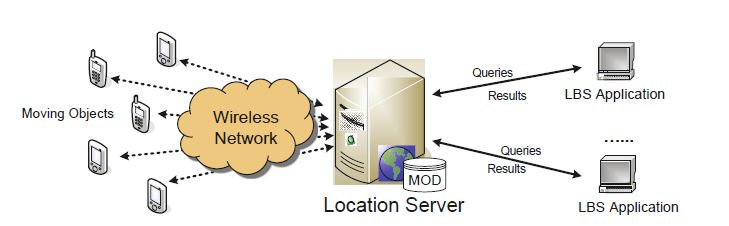
\includegraphics[scale=0.6]{LocationServer.JPG}

\caption{System model for locations based services}
\label{fig:system_model_for_locations_based_services}
\end{figure}


There are several options presented by \cite{Lee2011} how one can do data reduction and filtering techniques on spatial trajectories and thereby reduce the amount of data saved. There is batch compression (offline) and online algorithms for data reduction. Batch compression do computation on a full set of location points and then transmits it to the location server. Online algorithms computes directly on online selective data. In bikebus currently the following processing are implemented:
\begin{itemize}
    \item Douglas-Peucker compression algorithm
    \item Sliding Window compression algorithm
\end{itemize}

\begin{figure}[H]
\centering
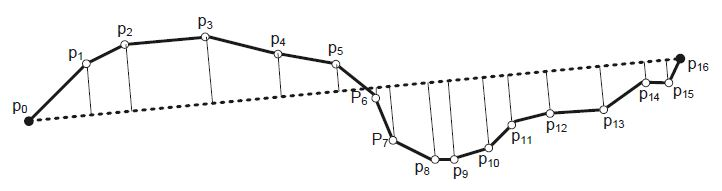
\includegraphics[scale=0.6]{DP.JPG}

\caption{Douglas-Peucker algorithm}
\label{fig:douglas_peucker_algorithm}
\end{figure}



\begin{figure}[H]
\centering
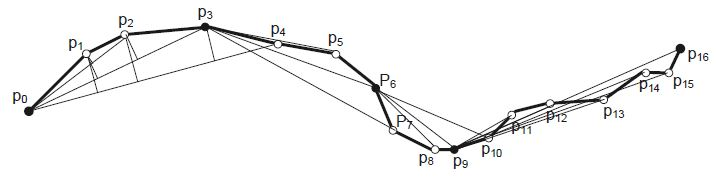
\includegraphics[scale=0.6]{SlidingWindow.JPG}

\caption{Sliding Window algorithm}
\label{fig:sliding_window_algorithm}
\end{figure}


Suggestions for further processing:
\begin{itemize}
    \item Median filtering
    \item Advanced statistics calculations (analyse per interval)
    \item Algorithm to balance the trade-off between processing space and time (Appendix \ref{app:processing_algorithm})
\end{itemize}


\section{Closing the Sensing Loop}
% TODO:
% Apply definitions
% Little introduction
% Explain concepts
%    - Sharing
%    - Privacy 
%    - Personalization
% Relate to articles
% Relate to app: 
%    - privacy: delete raw data after processing
% Reflect and discuss
        
%***************************************************************
%               Part 2: Architecture
%***************************************************************

\chapter{Architecture Qualities}
    %TODO:
% Apply defintiions
% Short introduction to Architecture qualities
As software engineers our focus is on creating a software architecture based on the architectural requirements. Software architecture allows us to reasons and take qualified decision. It is essential that we early in the project    \cite{un}

\section{Quality Attributes}
We will follow the definition on software architecture from \cite{Bass}. 
%**************************************Definition Software architecture
\begin{defi}[\textbf{Software architecture}]
The software architecture of a system is the set of \textbf{structures} needed to reason about the system, which comprise software \textbf{elements}, \textbf{relations} among them, and the \textbf{properties} of both. 
\end{defi}
%**************************************Definition Software architecture End

\noindent
Our approach towards implementing a software architecture is based on Quality attribute (QA) and Quality attribute scenario (QAS). A quality attribute (QA) according to \cite{Bass} is as follows.

%**************************************Definition Quality attribute
\begin{defi}[\textbf{Quality attribute}]
..A quality attribute is a measurable or testable property of a system that is used to indicate how well the satisfies the needs of its stakeholders..  
\end{defi}
%**************************************Definition Quality attribute End


% TODO:
% Introduction to QA
% List relevant quality attributes
% Why these attributes?
% Relate to generel mobile application challenges and tactics
\noindent
From \cite{Bass} we have seven quality attributes here among modifiability, availability and performance. Furthermore \cite{Kjaergaard:2015:AQT:2737182.2737196} has added energy efficiency and and ressources adaptability.  



\section{Quality Attribute Scenarios}
% TODO:
% Formal definition of QAS
% Use template from Bass
\noindent
A core observation is that a QA should be measurable or testable quality. The key point is when working with QA we use them in a given context/scenario and therefor we informally call these as QAS.\\



\begin{figure}[H]
\centering
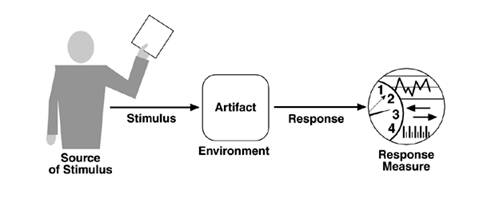
\includegraphics[scale=0.8]{QualityAttributeScenario.jpg}

\caption{The parts of a quality attribute scenario}
\label{fig:Quality_Attribute_Scenario}
\end{figure}





\noindent
One of the core aspects of the definition of software architecture, is that software architecture is a set of structures, which we can use to reason about the system. To assist and visualize these structures, elements, relations and properties we use Module-, Component \& Connector (C\&C)- and Allocation viewpoints \cite{3+1}. 

\begin{enumerate}
    \item Module viewpoint is concerned with how functionality of the system maps to static development units. The focus will be on elements such as classes and interfaces and relationships such as associations, generalizations, realizations and dependencies.
    \item Component \& Connector viewpoint is concerned with the runtime mapping of functionality to components of the architecture. Components are the executing things that perform a function. Connectors are the communication channels between components. The purpose is to focus on the flow of data and responsibilities such as a network call or method call etc.
    \item Allocation viewpoint is concerned with how software entities are mapped to environmental entities. Here the focus are on the physical stuff such as computer or a network. We specify the environment in order to make the software running. 
\end{enumerate}

\noindent
These viewpoint originates from $3+1$ article \cite{3+1}, where the $+1$ is the architectural requirements. These architectural requirements can be formulated through QAS.


\begin{table}[H]
\begin{center}
\begin{tabular}{|p{0.3cm}|p{2.5cm}|p{8cm}|}
  \hline
  \multicolumn{2}{|p{3cm}|}{\bfseries Scenario(s):} & \#  5: A developer should be able to make a change to the random number generator code under runtime and the change are made and tested within 3 hours. \\
  \hline
  \multicolumn{2}{|p{3cm}|}{\bfseries Relevant Quality Attributes:} & Modifiability\\
  \hline
  \multirow{6}{*}{\begin{sideways}{\bfseries Scenario Parts}\end{sideways}}
  & {\bfseries Source:} & Developer \\
  \cline{2-3}
  & {\bfseries Stimulus:} & Needs to replace the random generator \\
  \cline{2-3}
  & {\bfseries Artifact} &  Code \\
  \cline{2-3}
  & {\bfseries Environment:} &  Design time \\
  \cline{2-3}
  & {\bfseries Response:} &  Replacement made and Unit tested\\
  \cline{2-3}
  & {\bfseries Response Measure:} & In three hours\\
  \hline
\end{tabular}
\caption{Modifiability QAS}
\end{center}
\end{table}


\section{Tactics}
% TODO:
% For each QA find tactics
% Examples
%   - Performance: Limit sampling rate
%       - Possible solution: Our hierarachy divide and 
%         conquer
%   - Modifiability: Encapsulation/coupling/cohesion
%       - Possible solution: Interfaces, multiple APIs 
%         and storage
%   - Availability: Redundancy (caching layer)
%       - Possible solution: local caching

\noindent
We will discuss different tactics on software architecture for achieving the business goal for the electronic voting application. A tactic according to \cite{Bass} is defined as.

%**************************************Definition Tactic
\begin{defi}[\textbf{Tactic}]
Tactic is a design decision that influences the achievement of a quality attribute response. 
\end{defi}
%**************************************Definition Tactic End
    


\chapter{Solution Approach}
    %Anna

% Domain layer 
% Data layer (firebase)
% tactics
%  - interfaces and listeners (dependecy injection) (composite pattern?)
%  - activity recognition vs significant
%  - No Location - new model for calculations
% choice of tecnhologies and sensors

\section{Application Architecture}



\section{Continuous Sensing Architecture}

The continuous sensing in this application is formed from the notions of:
\begin{itemize}
    \item Geofence 
    \item Location 
    \item Activity Recognition
\end{itemize}

When the user creates or applies to a bikebus two Geofences are created for the start and end destination on the route. When the user is within the one of the Geofences, the Geofence fires an event which either initiates or stops the data collection.
Concretely the application holds a SensorDataController, which controls the flow of sensor data. 
\begin{enumerate}
    \item Creating two Geofence pending intents from the GoogleGeofence class
    \item The GeofenceIntentService class receives a GoogleGeofenceEvent object when a Geofence is triggered
    \item Based on the information from the Geofence event the GeofenceIntentService sends a status and result value back to the SensorDataController through a BroadcastReceiver
    \item The SensorDataController either stops the activity recognition or creates pending intents at a given sample rate from the GoogleActivityRecognition class
    \item Each time the ActivityRecognizeService class receives an intent with a ActivityRecognitionResult object the intent service broadcasts the results back to the SensorDataController
    \item Based on the activity has the value "ON\_BICYCLE" the SensorDataController will retrieve the current location of the user and store all locations for data processing
\end{enumerate}

\begin{figure}[H]
\centering
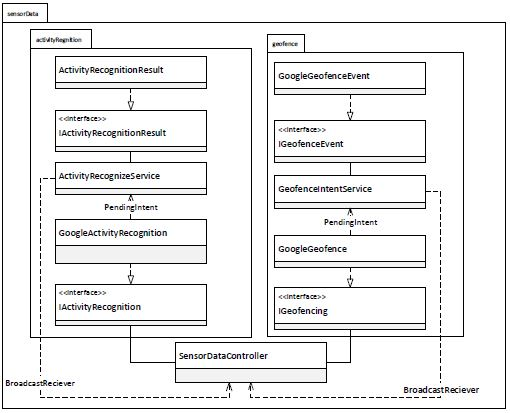
\includegraphics[scale=0.8]{Graphics/Images/Module_View_SensorData.jpg}
\caption{Module view of sensorData package}
\label{fig:Module_View_Sensor_Data}
\end{figure}
In figure \ref{fig:Module_View_Sensor_Data} a module view has been created based on the continuous data collection description. 

In Android there is typically two methods to apply when wanting to create background processes:
\begin{itemize}
    \item IntentService
    \item AsyncTask
\end{itemize}

The IntentService is a method used for long-term running background processes that is not dependent on the Activity. The AsyncTask is oppositely a method that only exists in the Activity's lifecycle, because it needs to return the value directly to the Activity. Therefore the AsyncTask cannot continue to run outside the application, and is more suited for short-term running background processes which are dependent on the Activity. 
\footnote{\url{https://github.com/codepath/android_guides/wiki/Starting-Background-Services}}

\section{Domain layer}

The domain layer of the application contains three central classes and two enum classes. In figure \ref{fig:domain_layer} below a class diagram have been constructed of those classes. 

\begin{figure}[H]
    \centering
    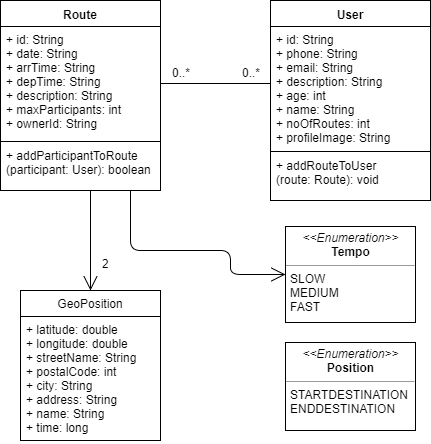
\includegraphics[scale=0.5]{Graphics/Images/domain_class_diagram.png}
    \caption{Class Diagram of Domain Layer}
    \label{fig:domain_layer}
\end{figure}

It can be seen that the "Route" and "User" classes have a tight relationship. Each route has a list of users as participants (excluding the owner), and each user has a list of created or applied to routes. This is a independent relationship, because a route can exist without any participants, and a user can exist without any routes created or applied to.

A "Route" contains two "GeoPosition" references as start destination and end destination.
The "GeoPosition" class can be instantiated by only latitude and longitude but also by the coordinates and an address. The address can be either a streetname, city and postal code, or if it is a public place i.e. "Odense Zoo" it can be name and and an address. The get methods will automatically return the correct data regardless of the construction, including potientially calculating the address from only coordinates using the static "AddressService" class which uses the "Geocoder" library.

The "Tempo" enum class is used to denote the tempo of a given route. Currently the user chooses the tempo subjectively when creating a route, but an idea for future work is to calculate the tempo automatically based on the distance and the guiding duration.

The "Position" enum class is currently only used when handling geo-fences in the data collection to determine whether the activated geo-fence is a start or end destiantion.

\section{Graphical User Interface}
The graphical design of this application is strongly inspired from another app called "GoMore", which has the concept of coordinating carpools. The "GoMore" concept reminds a lot about the "BikeBus" concept, because both apps coordinates for friends and strangers to ride with each other. The main differences between the two concepts are that "BikeBus" coordinates free bicycle rides and paid "GoMore" coordinates Car rides.

The graphical user interface of the application is developed using the Android API, which connects each view with an activity. In figure \ref{fig:activities} below a diagram shows the connections between each activities, where the dotted line represents the navigation between views using the "startActivity" method, and the other arrows follows UML by showing inheritance and association between the classes.   

\begin{figure}[H]
    \centering
    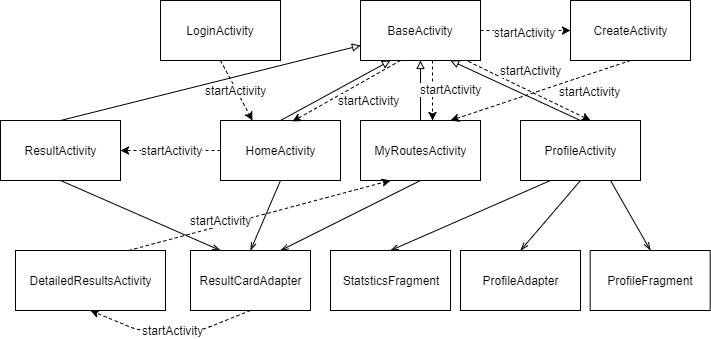
\includegraphics[scale=0.5]{Graphics/Images/Activity_Diagram.png}
    \caption{Diagram of activities}
    \label{fig:activities}
\end{figure}

As it can been seen in the figure, four activities inherits from the "BaseActivity" class, which sets the bottom navigation bar and the floating create button. The create button is though removed from the "ProfileActivity". 
This structure collects the base functionalities for some of the activities to make it easily modifiable.
Beside from the activity classes, the diagram also contains fragment and adapter classes. The two fragment classes "ProfileFragment" and "StatisticsFragment" coexists with the "ProfileAdapter" class to create a tab view, where the user can switch between profile and statistics information in the same activity. The "ResultCardAdapter" is used by three different activities because it implements a generic way of presenting a list of information viewed as "cards" in the material design. These cards are used in the "HomeActivity" as a list of recent routes, the "ResultActivity" as a search result list of routes, and the "MyRoutesActivity" as a list of routes created of applied to by the user. Again this adapter work generically, making it possible for multiple activities to use the functionality in different cases easily.

\subsection{Data Layer}
\label{sec:data_layer_design}

In order to create and search through routes across multiple devices and users, a database must be created to store all route and user information.
We have chosen to create the database in Firebase, which is a real-time document database hosted by Google. As Firebase is hosted by Google online it is therefore server-less and easy to setup and manage. On the other the application cannot retrieve data offline, and it becomes quite inconvenient to create a manual caching layer. Firebase is a NoSQL database, which means all querying has to be done manually. Firebase only returns a "snapshot" of the data at a given place in the database, and that should be information enough making querying disposable. This simple database structure becomes very scalable and performs very well for retrieval, which typically is the main requirements for real time mobile applications.

Firebase stores JSON trees of strings, which can easily be serialized into objects in Java. Best-practices of these JSON trees are to make the tree as flat as possible with references to objects. If the JSON tree is too deep and contains multiple layer of nested objects, the data snapshot retrieved for the application becomes very large and possibly very extravagant. Therefore it is more efficient to store a list of each object type containing meta data and a reference to possibly nested objects to be looked up in another data snapshot.

% Why store google account data when already logging in with google?
Currently our database looks as the following:
\begin{figure}[!htb]
    \centering
    \begin{minipage}{.5\textwidth}
        \centering
        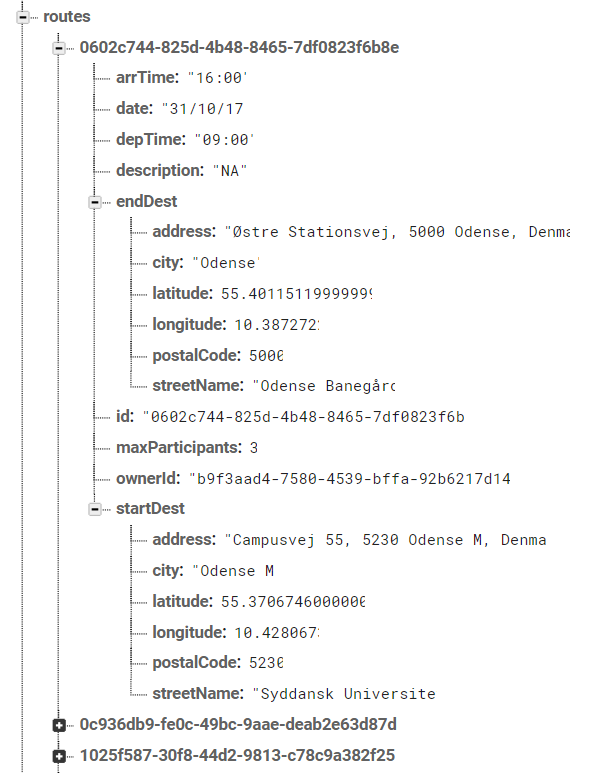
\includegraphics[scale=0.8]{Graphics/Images/firebase_routes.PNG}
        \caption{Route objects in Firebase}
        \label{fig:firebase_routes}
    \end{minipage}%
    \begin{minipage}{0.5\textwidth}
        \centering
        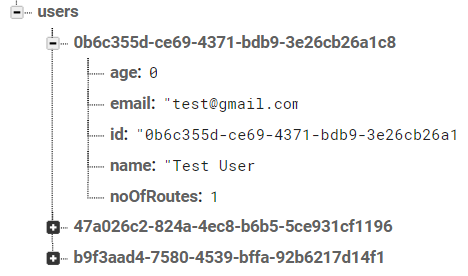
\includegraphics[scale=0.8]{Graphics/Images/firebase_users.PNG}
        \caption{User objects in Firebase}
        \label{fig:firebase_users}
    \end{minipage}
\end{figure}

Each route has a GUID key which can be referenced from other objects. For instance does each route contain a user reference as "ownerId". The "startDest" and "endDest" values could also be created as references to a new GeoPosition object in Firebase to reduce tree depth and avoid redundant data.
Connecting participants to a route is not implemented yet, but it would have been done as a "participant" list of user references for each route to maintain the flat tree structure. Changes in these objects has to be reflected in the domain classes, because the data snapshot automatically serializes the objects to a defined class structure. Therefore the data structure is a trade-off between best-practices of the firebase structure and the domain class structures.

The data retrieval is implemented in the "FirebaseDbHelper" class which implements a defined "IStorage" interface using the listeners "OnGetRoutesListener" and "OnGetUsersListener" due to asynchronous data retrieval. This structure is setup as modular as possible to ensure the database easily can be replaced with different technologies or database types. 

\subsection{Design}
The "BikeBus" application follows the "Material Design" principles created by Google\footnote{\url{https://material.io/guidelines/#}}, which are quite popular for Android apps. Material Design has great guidelines on how to improve mobile user experience and can quickly make the application look more professional.

The Android GUI components used to provide the Material Design elements:
\begin{itemize}
    \item CardView - The card element containing information of the bikebus
    \item RecyclerView - Infinity scroll view containing only cardviews
    \item BottomNavigationView - The bottom navigation menu between search, routes and profile tabs
    \item TabLayout with ViewPager - A Tab view in the profile view which switches between the profile and statistics fragment
    \item FloatingActionButton - The red create button
\end{itemize}

In this project Google API's has been frequently used for especially sensor data, but the Google AutoComplete

\begin{figure}[!htb]
\centering
\begin{minipage}{0.32\textwidth}
\centering
    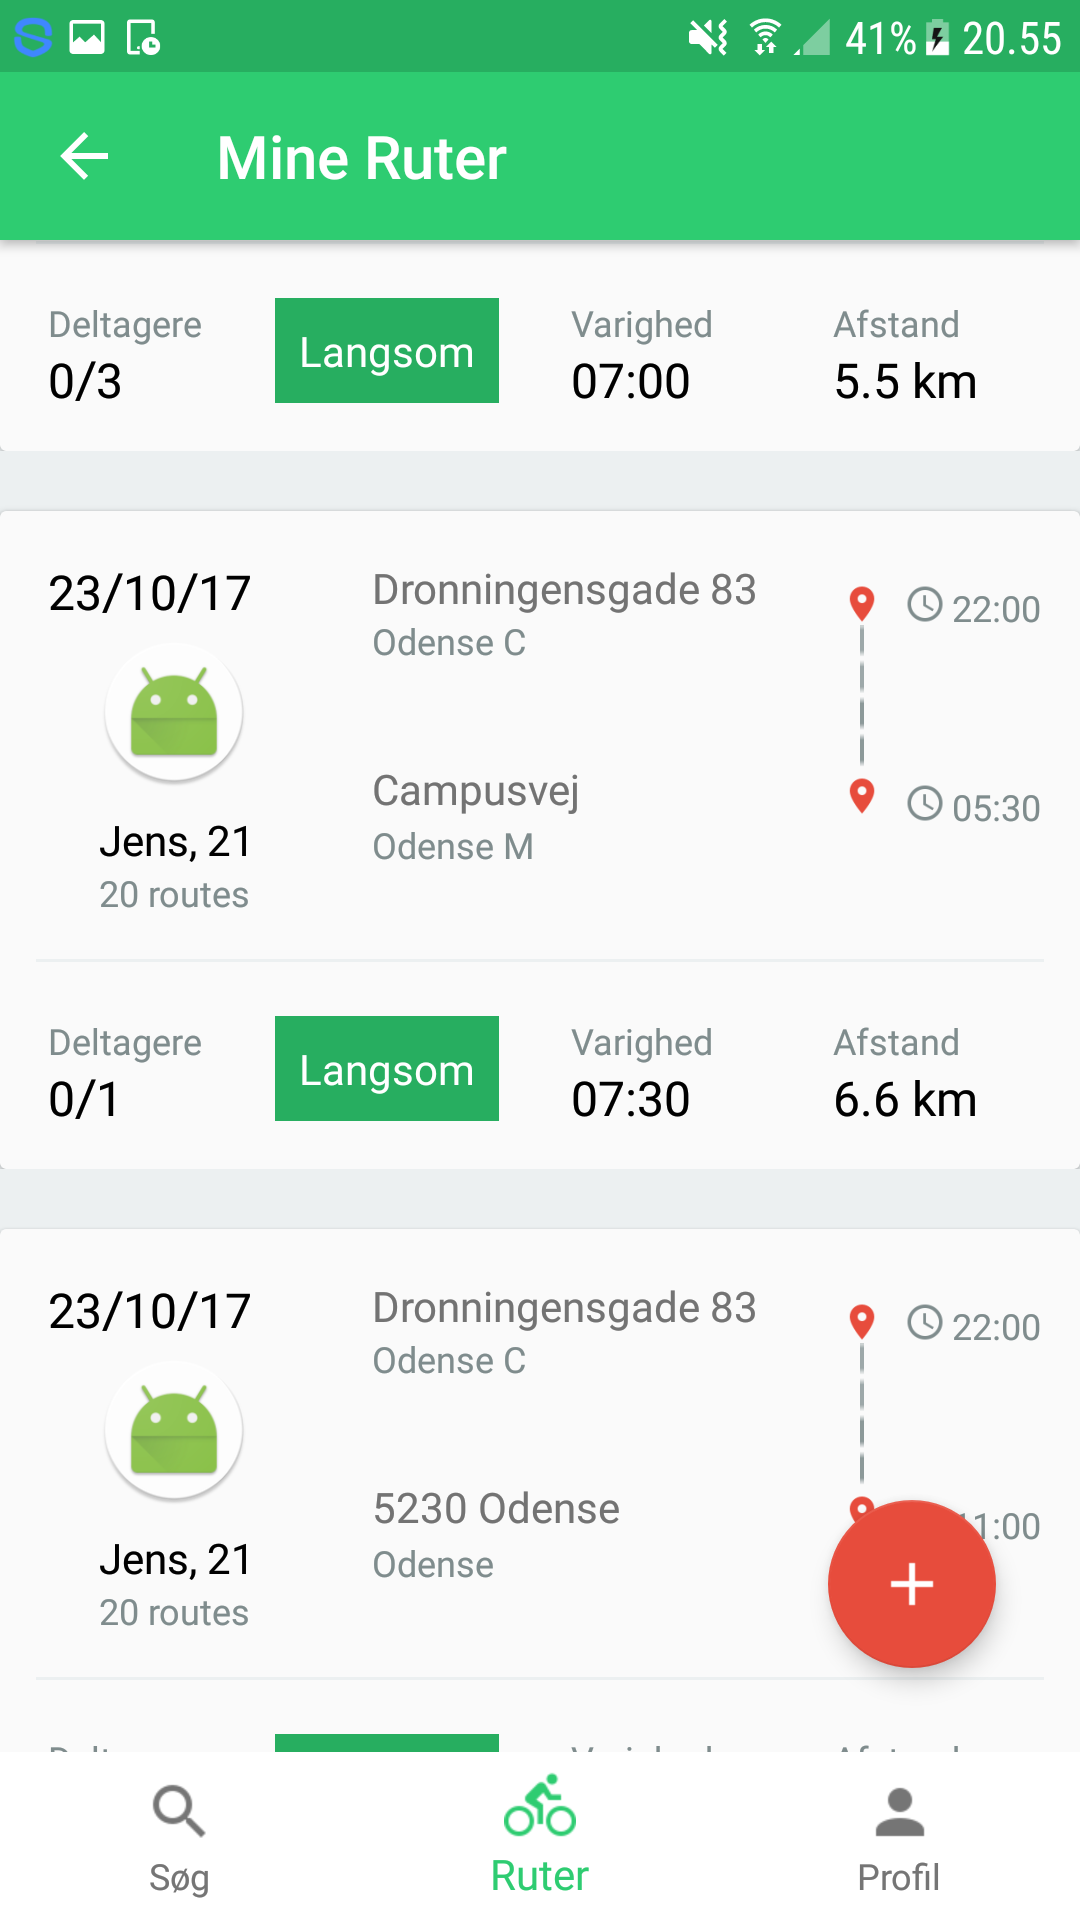
\includegraphics[width=\linewidth]{Graphics/Images/bikebus_search.png}
    \caption{Result page for BikeBus}
    \label{fig:sample_figure}
\end{minipage}\hfill
\begin{minipage}{0.32\textwidth}
\centering
    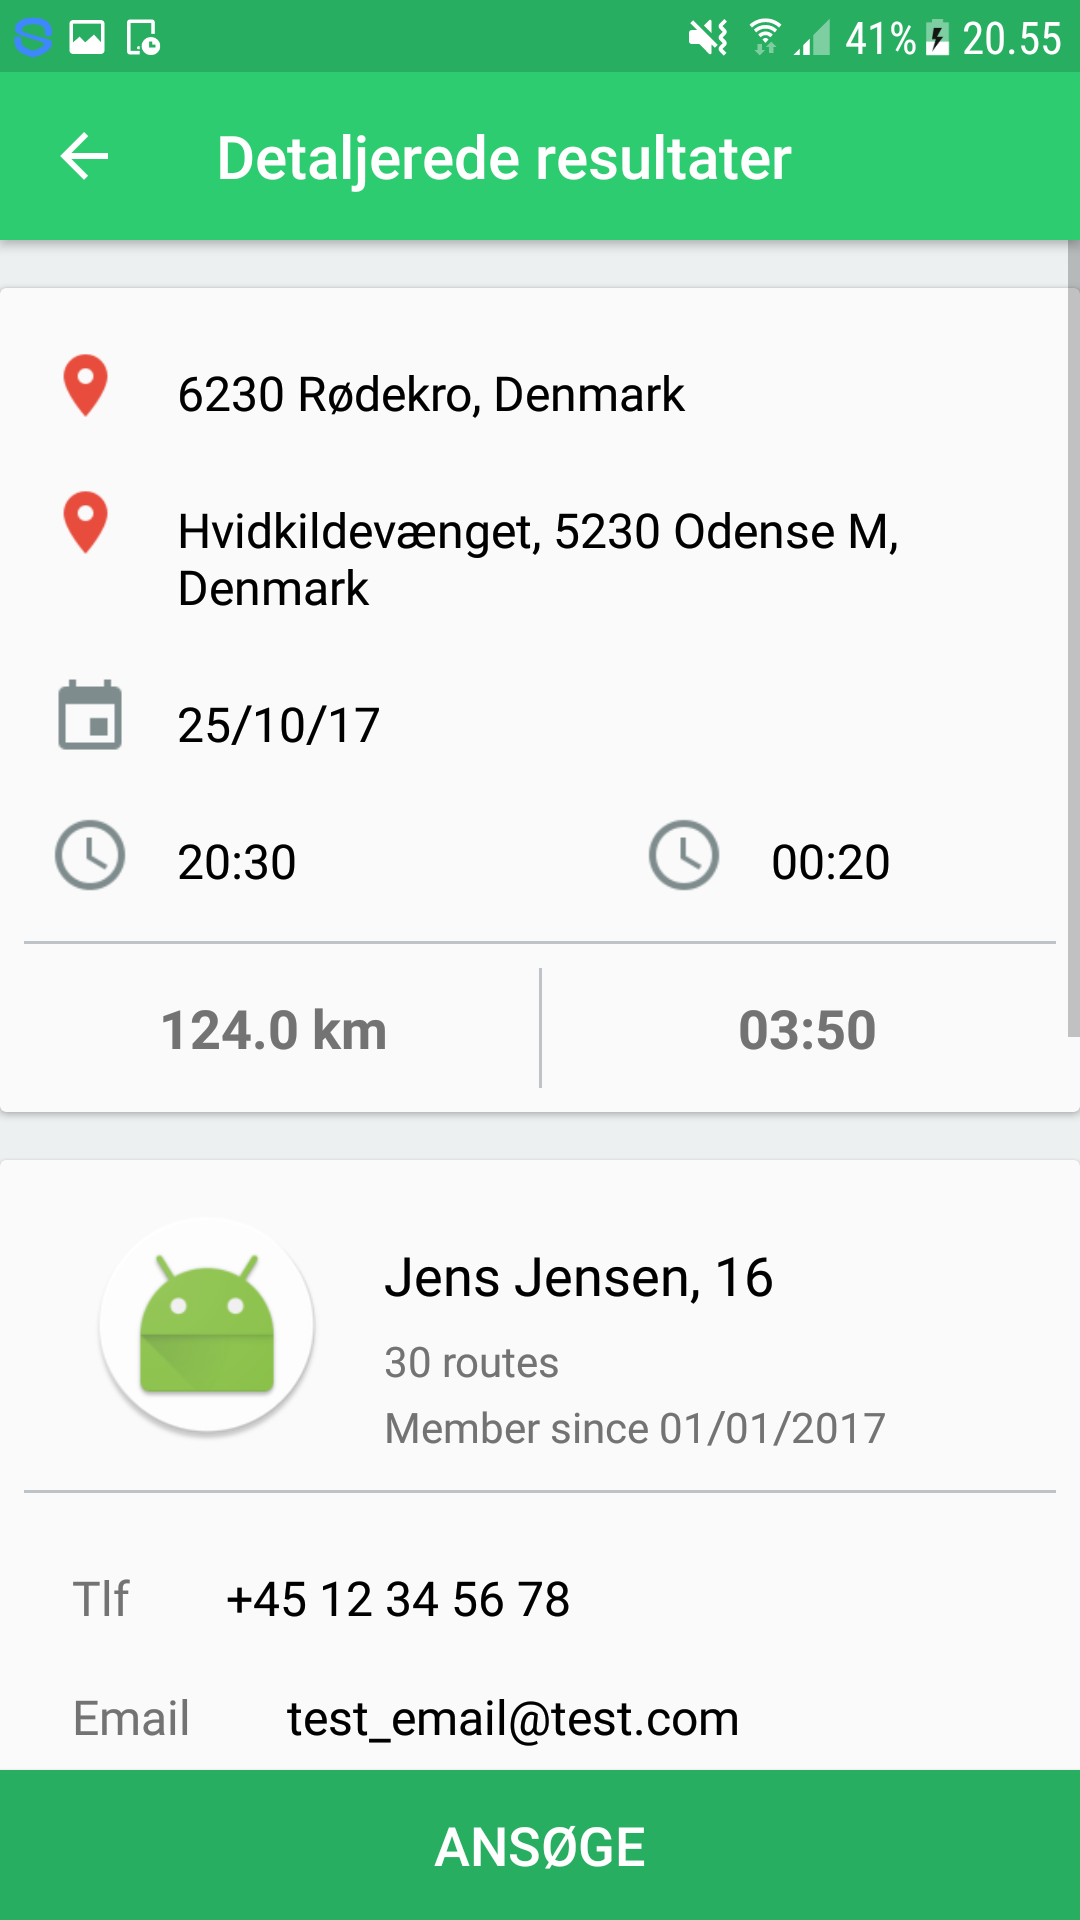
\includegraphics[width=\linewidth]{Graphics/Images/bikebus_detail_1.png}
    \caption{Detailed page for BikeBus (part 1)}
    \label{fig:sample_figure}
\end{minipage}\hfill
\begin{minipage}{0.32\textwidth}
\centering
    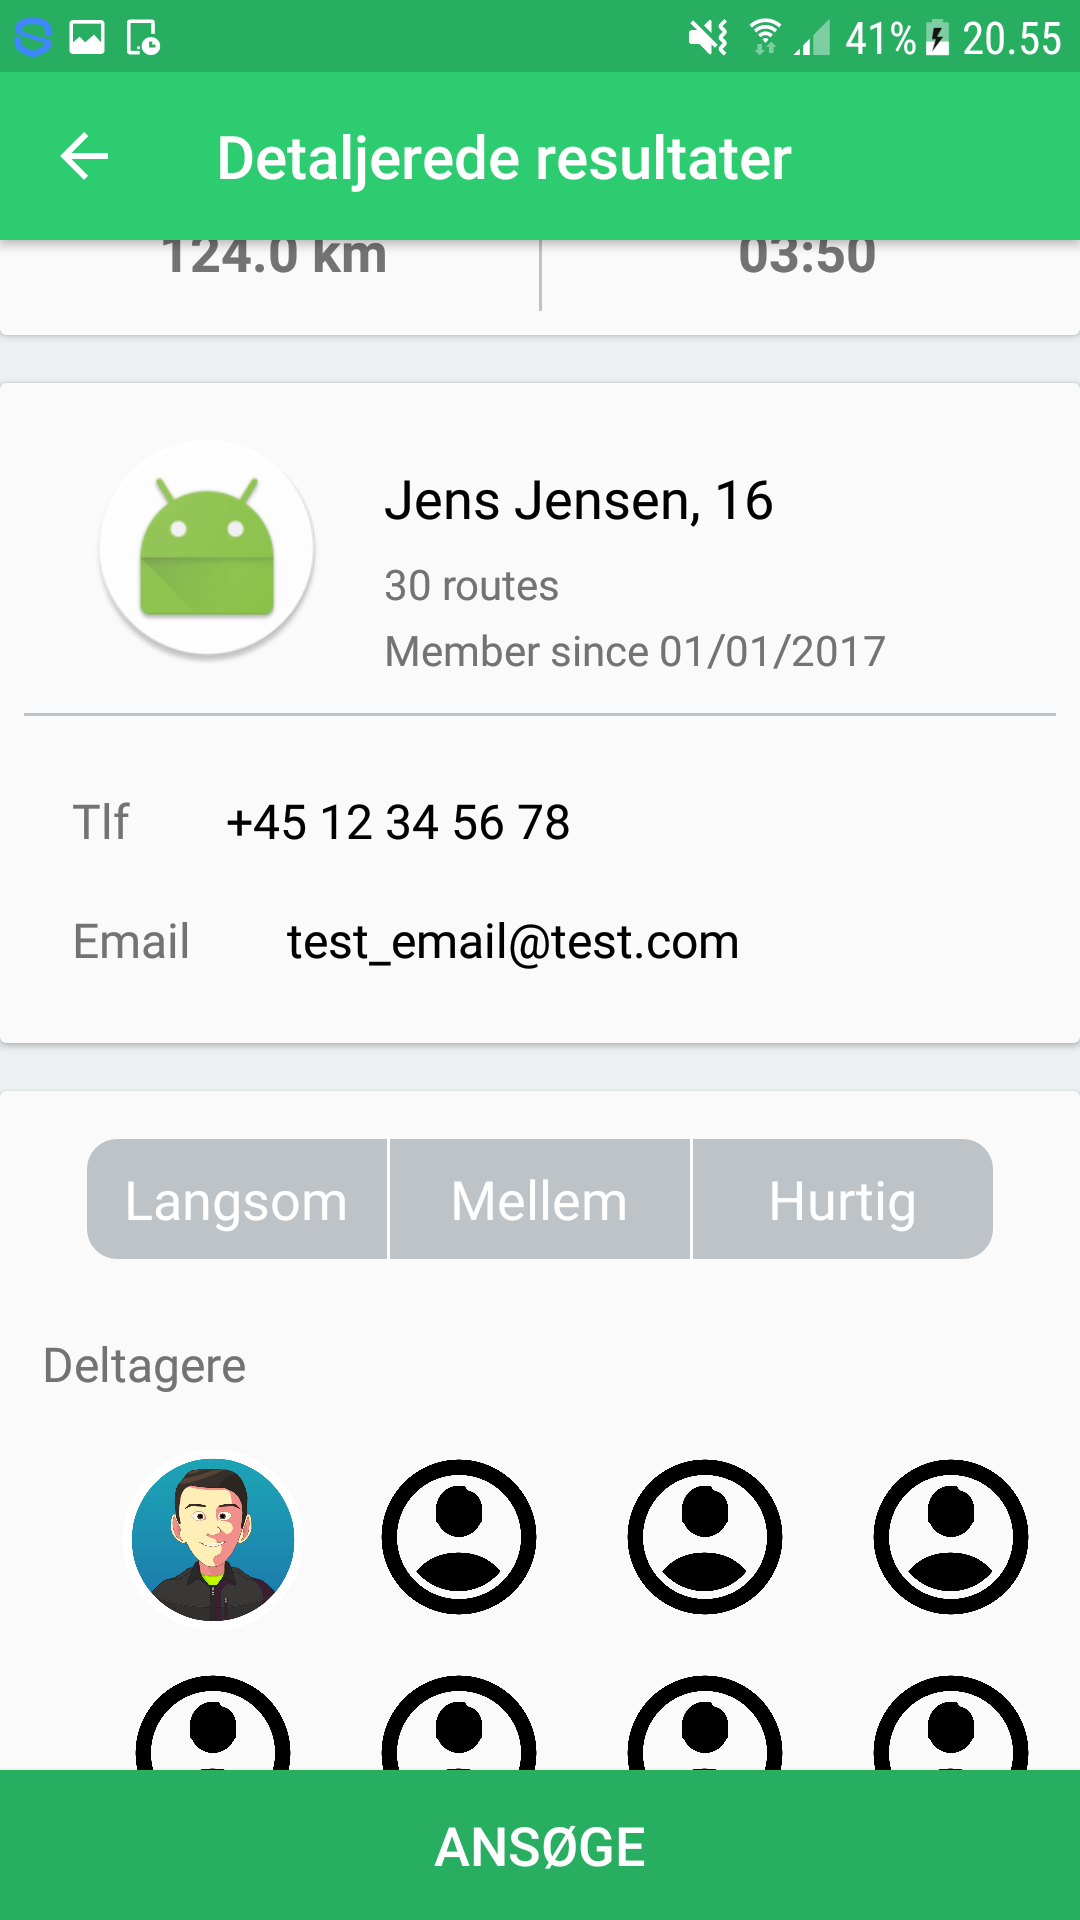
\includegraphics[width=\linewidth]{Graphics/Images/bikebus_detail_2.png}
    \caption{Detailed page for BikeBus (part 2)}
    \label{fig:sample_figure}
\end{minipage}
\end{figure}

\chapter{Solution Description}
    % Admir, Anna,  Sune (prototype)

% API implementation - Google, Firebase, Activity Recognition (Admir)
% Data Collection - Geofence, Activity Recognition, Location (Sune) - blir det ikke forklaret i section 5.2
% Search (Sune)
% Distance calculator
% ILocation and IStorage or other with interface and listener
% Adapter view pattern (Anna)

% TODO:
% Apply definitions
% Introduction
% Explain three different categories of prototyping
%    - Explorative, Experimental, Evoulutionary


In the following sections, central aspects of the Bikebus solution will be highlighted. This are applied examples on compression techniques and examples of architectural designs. 

% TODO:
% Explain all protoypes in our program (Implementation)
%    - Datastructures, algorithms, storage, etc
%    - Diagrams
%    - Results of prototypes

% Current Prototypes:
% - Easily shift sensor API (modifiability) 
%    - EmotionSenseLocation.java and ILocation  
% - SQLite for internal storage (availablity)


% Prototypes:
\section{Compression}
One of the features which needs to implemented in Bikebus is the compression functionality of locations points. Three prototypes have been made separate from the application which are illustrated in following examples. All examples are done in Python and plotted with Leaflet.  

Figure \ref{fig:route_without_filter} illustrates a clip of the raw data of a biking route. The route consists of 630 location points. On figure \ref{fig:route_with_filter} the median filter is applied on same route. By applying the median filter result in a much more smooth route, with less outliers/noise, which is described in section \ref{sec:data_processing}. 
\begin{figure}[H]
\centering
\begin{minipage}{0.50\textwidth}
\centering
    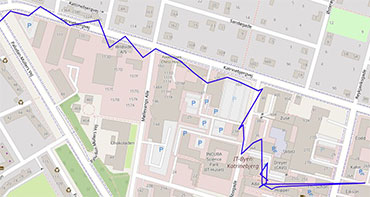
\includegraphics[width=\linewidth]{RouteWithOutFilter2.jpg}
    \caption{Without median filter}
    \label{fig:route_without_filter}
\end{minipage}\hfill
\begin{minipage}{0.50\textwidth}
\centering
    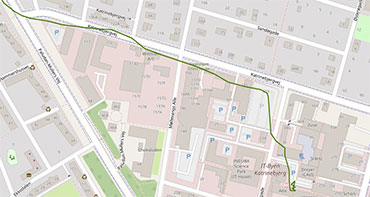
\includegraphics[width=\linewidth]{RouteWithFilter2.jpg}
    \caption{With median filter}
    \label{fig:route_with_filter}
\end{minipage}
\end{figure}

To get a better overview, both of the following maps are rotated. The DP compression is applied on figure \ref{fig:douglas_peucker_compression}. After applying the DP the routes is compressed to 20 location points. Figure \ref{fig:sliding_window} shows the route after applying Sliding window. For this prototype the code simulates how location points arrives periodically to be processed by the Sliding window algorithm. The compression results in 304 location points, which is $50\%$ compression of the original route.

\begin{figure}[H]
\centering
\begin{minipage}{0.50\textwidth}
\centering
    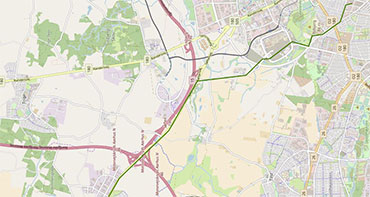
\includegraphics[width=\linewidth]{RouteDP2.jpg}
    \caption{Douglas Peucker compression (offline)}
    \label{fig:douglas_peucker_compression}
\end{minipage}\hfill
\begin{minipage}{0.50\textwidth}
\centering
    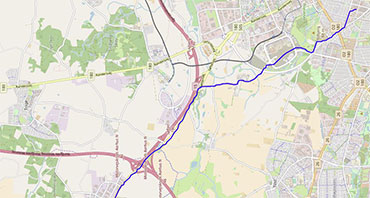
\includegraphics[width=\linewidth]{RouteSW2.jpg}
    \caption{Sliding window compression (online)}
    \label{fig:sliding_window}
\end{minipage}
\end{figure}

Since the core engine of Bikebus is build on a flexible architecture, it should be manageable to plug these algorithms into Bikebus. When pluggin compression algorithm into Bikebus more testing has to be done on how it affects the energy consumption.

Figure \ref{lst:sliding_window_code} is an implementation of the sliding window. Basically it follows the steps described in figure \ref{fig:sliding_window_algorithm}. To achieve the open window algorithm one only needs to change the point added to the approximated trajectory and the new anchor point. As described in figure \ref{fig:open_window_algorithm} the open window chooses the point with largest distance when the threshold is violated.      

\lstinputlisting[label={lst:sliding_window_code}, caption={Sliding window}, language={Python}]{Graphics/Images/SlidingWindow3.py}

\section{Module viewpoint of the distance calculation}
By encapsulated the distance calculation, the system is robust to changes. The first implementation was the simple distance calculator which consist of a primitive euclidean distances calculation. Later when the Google API was integrated the Google distance matrix was implemented. By using a strategy pattern \cite{Baerbak10} it was easy to implement the new calculator without breaking existing functionality. 

\begin{figure}[H]
\centering
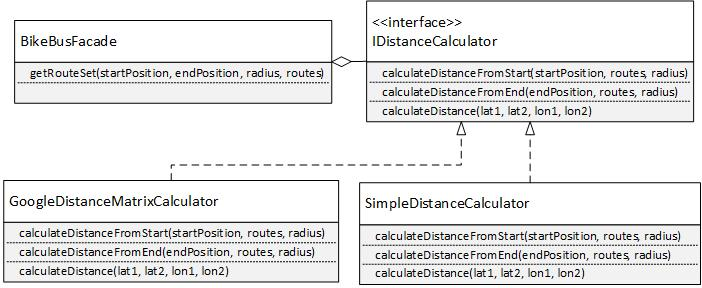
\includegraphics[scale=0.6]{Distance.jpg}
\caption{Module viewpoint of the strategy pattern of distance calculation}
\label{fig:module_view_distance_calculation}
\end{figure}

\section{Module viewpoint of the activity recognition and location}
As stated in section \ref{subsec:modifiability} the encapsulation tactic was chosen to achieve modifiability on replacing the sensor framework. The encapsulation is realized by coding to small interfaces and thereby achieving low coupling and high cohesion. Figure \ref{fig:activity_regonition_module_viewpoint} is a rough overview of the relations between the core classes gathering sensor data when biking.  
Notice that every class is encapsulated behind an interface. This also holds true for the activity recognition package seen in figure \ref{fig:Module_View_Sensor_Data}. It should be durable to hold the response measure by doing change by addition \cite{Baerbak10}.    

\begin{figure}[H]
\centering
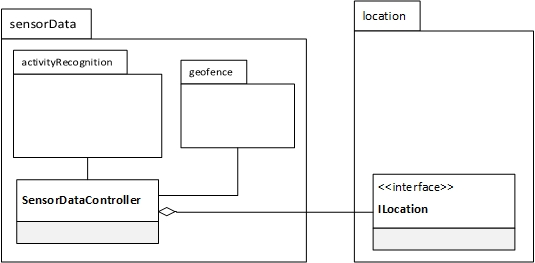
\includegraphics[scale=0.6]{ActivityRegonitionModuleViewpoint.jpg}
\caption{Module viewpoint of sensorData and location package}
\label{fig:activity_regonition_module_viewpoint}
\end{figure}
%***************************************************************
%               Part 8: Related work
%***************************************************************
\chapter{Related Work}
    % TODO:
% Collect all articles 
% Describe related apps (GoMore, CykelScore, ...)
% UX material design
% Other resources
%***************************************************************
%               Part 9: Reflection 
%***************************************************************
\chapter{Reflection and Discussion}
    %(All)

% TODO:
% Overall evaulation and discussion
%***************************************************************
%               Part 9: Conclusion
%***************************************************************
\chapter{Conclusion}
    % Conclusion (Sune)

% TODO:
% Conclusion, Perspective, Future Work

% Problem
% - Increase safety for kids
% - Coordination of bikebus
%    - App
% - Mobile sensing
% - From schools perspective younger and older kids together
%    - group implementation

% - Usability for kids using the app!
%   - community sharing if many uses
% - Social aspects
% - Modifiability -> new features added quickly with high reliability -> app is more attractive -> more users -> more useful information (for community)

% - Current State (qualities)
%   - Mobile Sensing 
%   - Create, apply, search, profile functionalities
%   - Google APIs -> attractiveness -> modifiability of technologies
%   - Focus on good Architecture! (interfaces, listeners, best-practices, design patterns)
%      - Ensure quality
%   - Compression
In this project, we presented a BikeBus mobile sensing application to address how mobile sensing and coordination can be used between kids biking. Basic functionality for coordination such as create, search and assigning routes is achieved, allowing kids to bike together. BikeBus should be a user friendly and an intuitive application for kids and therefore time was invested in working with flow and the graphics in the initial phase. Different sensors is discussed, explored and implemented to pull accurate location data. BikeBus uses standard implementation of Google API's for location data, activity recognition and geofence.

Working with location based system, challenges such as data privacy and data gathering needs to be addressed. When transferring from individual sensing to a community based sensing, different data privacy techniques should be considered. Several techniques for compressing sensing data has been presented and applied. Initial findings shows that the median filter should be applied before running off-line algorithms. Both off-line and on-line results in compression savings of 50\% (on-line) and 96\% (off-line).

Different techniques for architecting mobile application has been applied, for achieving measurable demands and high quality of code. QAS has been defined for both energy and resource adaptability which addresses fundamental challenges regards to mobile applications. The proposed tactics has been identified for each of the QAS. The energy consumption has been monitored and the test shows that BikeBus holds the response measure. Modifiability has been prioritized in much of the code work applied to BikeBus. One off the core aspect for this application is being able to change the sensor framework with another. The work with resource adaptability illustrates that there is always trade off which has to be considered. In this example its about accuracy and availability.    


By applying known software design principles such as coding to interfaces, low coupling and high cohesion, results in a modifiable architecture. BikeBus should be attractive and new as old users should keep using the application. One way for achieving that is by continuing being able to add new features to the application in a reliable way.   

\subsection{Future Work}
By having a flexible architecture allows us to easily extend to group functionality, hereby being able to create private and public groups. This also implicates applying the presented privacy techniques. 

Parent notification is another feature which allows the parents to be notified when their children has arrived to their end destination. Visualizing real-time maps would allow participants to get a more precise knowledge about the other participants before starting the bike route.     

A lot of work has been put into experimenting with the compression algorithms. But more work on tuning and testing the implemented algorithms would be recommended.

The proposed QAS and corresponding tactics needs more investigation. Even though there is literature on these subjects, describing the challenges it is time consuming to apply. There is always trade off involved, regarding to performance versus accuracy.  This is also holds true for the presented compression techniques.

Further work should also consider to prioritize test coverage of the codebase. The fundamental for testability ought to be in place, since the codebase is build upon compositional design patterns.  

% Group (school group -> safety) - solve part of problem formulation
% Parent notification when arrival - solve part of problem formulation
% Visual aspects (Google Maps + evt real-time map when meeting) - provide more usability -> good app
% More work on energy results - increase quality
% More work on resource adaptability - increase quality

\subsection{Perspective}
Mobile applications which have had a lot of success as a long-term popular application have typically released new features frequently. An example of that the social application Snapchat, which started out as a basic picture sharing app, but today has integrated facial recognition features just for fun. These new complex features are in our opinion the main reason the app was not short lived as the Pokemon Go app. It should be quick to integrate new features to the existing app.

Another view point is mobile application which are popular because of their simplicity and enhanced user experience. Applications as MobilePay and Uber are both known for being so easily manageable, that anyone can use the app right after installation. The application should not provide the user with too many choices, it should lead the way, by for instance also limit the number of views to perform a function. 
Furthermore Uber has a real-time map showing the drivers position until pick-up. This feature is enhances the user experience by giving the user an overview instead of being dependent on the application only. 

As referenced to in the introduction the CykelScore application also has the purpose of motivating people (and especially children) to bike more often. Our application has the same purpose, but focuses more on usability and modifiability to keep users interested instead of gamification.

% Good App:
% - Outlook to other apps (snapchat, uber, gomore)
%   - Analyse why they are still popular
%   - New features (modifiability), usability (UX design - looks professional)
%   - Visual overview! (real-time where people are when meeting) - Uber
%   - Resource adaptability: Offline db so users still can see data offline (implemented on popular apps)
% - Read other papers (research)

%***************************************************************
%               Bibliography
%***************************************************************
\addcontentsline{toc}{chapter}{\\BIBLIOGRAPHY}
\bibliographystyle{alpha}
\bibliography{901_Bibliography}

\clearpage
%***************************************************************
%               Appendex
%***************************************************************
\appendix
\addcontentsline{toc}{chapter}{\\APPENDICES}
\chapter{Proofs}
% \section{Suggested Processing Algorithm}
% \label{app:processing_algorithm}
% An idea for minimizing temporarily storage of collected data is to apply the divide-and-conquer technique:
% \begin{itemize}
%     \item Define a static length of a data collection array (or other data structure)
%     \item When the array is full call online processing on that array asynchronously and continue data collecting into the same array
%     \item The result of each processing will be saved as one element in a new intermediate array with same static length as the first array
%     \item This processing strategy continues until the data collection is finished
% \end{itemize}

% Using this algorithm the temporarily storage will have the total space of $O(m*log_m(n))$, and the time consumption of the processing will be $\sum_{i=1}^{log_m(n)}{m^i}$, but parted into $\sum_{i=0}^{log_m(n)-1}{m^i}$ asynchronous calls <<Apply Tactics>>. The larger value the m variable have the more improved the runtimes get.

% \textbf{Example}
% Given $m_1 = 20$ elements and $m_2 = 3$ elements on a total of 8000 elements.
% Space consumption: 
% \begin{itemize}
%     \item $O(m_1*log_{m_1}(n)) = 20*3 = 60$ elements
%     \item $O(m_2*log_{m_2}(n)) = 3*8 = 24$ elements
% \end{itemize}

% Time consumption:
% \begin{itemize}
%     \item $\sum_{i=1}^{log_{m_1}(n)}{m_1^i} = 20+400+8000 = 8420$ elements to process
%     \item $\sum_{i=0}^{log_{m_1}(n)-1}{m_1^i} = 1+20+400 = 421$ process calls
%     \item $\sum_{i=1}^{log_{m_2}(n)}{m_2^i} = 3+9+27+81+243+729+2187+6561 = 9840$ elements to process
%     \item $\sum_{i=0}^{log_{m_2}(n)-1}{m_2^i} = 1+3+9+27+81+243+729+2187 = 3280$ process calls
% \end{itemize}

% This shows the size of m have the largest effect on number of process calls.
% Without this algorithm the space consumption would be $O(n) = 8000$ elements and time consumption would be $O(n) = 8000$ elements to process within $O(1) = 1$ process call.


%----------------------------------- Interface Figure
\subsection{Interfaces}
\label{app:interfaces}

\begin{figure}[H]
    \centering
    \hspace*{-1.73in}
    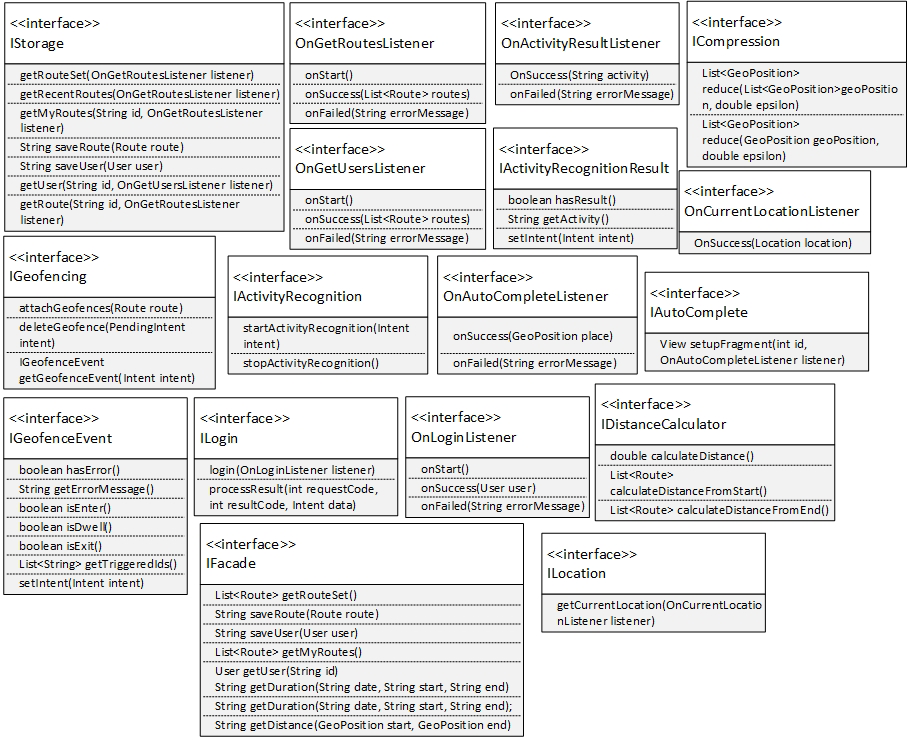
\includegraphics[scale=0.65]{Graphics/Images/Interfaces.png}
    \caption{Class diagram of interfaces}
    \label{fig:interfaces}
\end{figure}


%----------------------------------- Firebase Figures
\subsection{Firebase Structure}

\label{app:firebase_figures}
\begin{figure}[H]
    \centering
    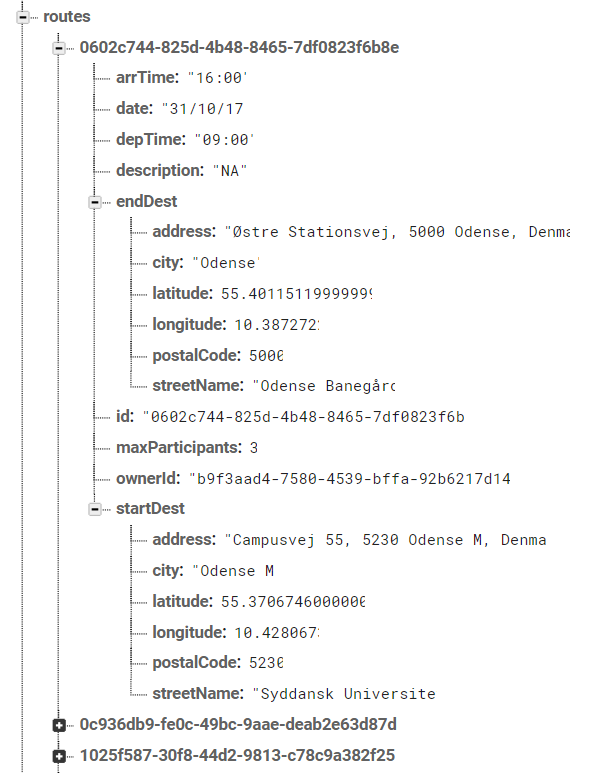
\includegraphics[scale=1.5]{Graphics/Images/firebase_routes.PNG}
    \caption{Route objects in Firebase}
    \label{fig:firebase_routes_appendix}
\end{figure}

\begin{figure}[H]
    \centering
    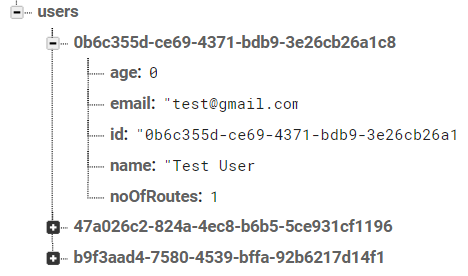
\includegraphics[scale=1.5]{Graphics/Images/firebase_users.PNG}
    \caption{User objects in Firebase}
    \label{fig:firebase_users_appendix}
\end{figure}


%----------------------------------- Compression Figures
\subsection{Compression}
\label{app:compression}

\begin{figure}[H]
    \centering
    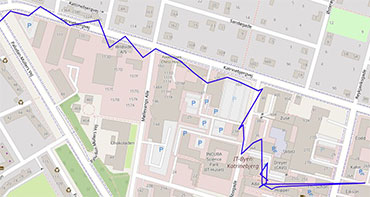
\includegraphics[scale=1.0]{RouteWithOutFilter2.jpg}
    \caption{Without median filter (blue line)}
    \label{fig:route_without_filter_appendix}
\end{figure}

\begin{figure}[H]
    \centering
    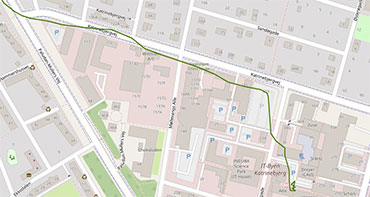
\includegraphics[scale=1.0]{RouteWithFilter2.jpg}
    \caption{With median filter (green line)}
    \label{fig:route_with_filter_appendix}
\end{figure}

\begin{figure}[H]
    \centering
    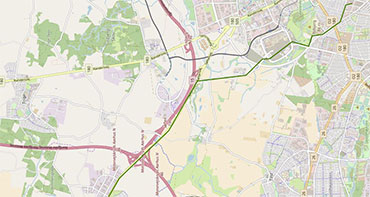
\includegraphics[scale=1.0]{RouteDP2.jpg}
    \caption{Douglas Peucker compression (green line)}
    \label{fig:douglas_peucker_compression_appendix}
\end{figure}

\begin{figure}[H]
\centering
    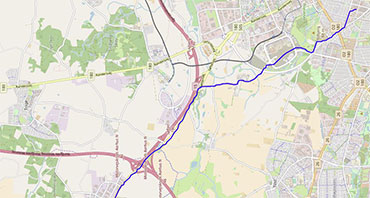
\includegraphics[scale=1.0]{RouteSW2.jpg}
    \caption{Sliding window compression (blue line)}
    \label{fig:sliding_window_appendix}
\end{figure}


\end{document}
